\section{Method}

\begin{frame}
    \frametitle{Problem Statement}

    \begin{itemize}
        \item Agent searches scene \(S \subset \mathbb{R}^d\).
        \item Scene contains set of targets \(\{t_0, \dots t_n\}\), \(t_i \in S\).
        \item Agent perceives view \(V \subset S\).
        \item View can be transformed to new subspace.
        \item Indicate when targets are visible, i.e. \(V \cup T \neq \varnothing\). 
        \item Maximize the probability of finding all targets while minimizing cost in time (NP-complete~\cite{andreopoulos_theory_2009}). % intractable to solve optimally
    \end{itemize}
\end{frame}

\subsection{Environments}

\begin{frame}
    \frametitle{Environments}
    
    \begin{itemize}
        \item Three simulated environments used for experiments.
        \item Search space discretized into \(H \times W\) camera positions.
        \item Each camera position has a unique view \(V \subset S\).
        \item Three targets in all scenes.
        \item Target probability correlated with scene appearance.
        \item Possible to do better than exhaustive search on average.
        \item Scenes procedurally generated:
        \begin{itemize}
            \item Pseudorandom seed determines scene appearance and target positions.
            \item Gives control over difficulty to solve.
            \item Can vary training and test set sizes by limiting seed pool.
        \end{itemize}
    \end{itemize}
\end{frame}

\begin{frame}
    \frametitle{Observation, Action and Reward}

    \begin{itemize}
        \item Observations \(o_t = \left\langle x_t, p_t \right\rangle\), where
        \begin{itemize}
            \item \(x_t \in \mathbb{R}^{3 \times 64 \times 64}\) is RGB image,
            \item \(p_t \in \{0, \dots, H-1\} \times \{0, \dots, W-1\}\) is camera position.
        \end{itemize}
        \item Actions \(a_t \in \{\texttt{INDICATE}, \texttt{UP}, \texttt{DOWN}, \texttt{LEFT}, \texttt{RIGHT}\}\), where
        \begin{itemize}
            \item \texttt{INDICATE} identifies targets, and
            \item \texttt{UP}, \texttt{DOWN}, \texttt{LEFT}, \texttt{RIGHT} move camera.
        \end{itemize}
        \item Reward \(r_t = h - 0.01 + 0.005d + 0.005e\) where
        \begin{itemize}
            \item \(h = \left\vert T \cap V \right\vert\) if \(a_t = \texttt{INDICATE}\), else \(0\).
            \item \(d = 1\) if \(a_t\) moves closer to nearest target, else \(0\).
            \item \(e = 1\) if \(a_t\) moves to new position, else \(0\).
            % rewarded for finding targets, moving towards them and exploring environment.
            % constant penalty encourages quick episode completion.
        \end{itemize}
    \end{itemize}
\end{frame}

\begin{frame}
    \frametitle{Environment I: Gaussian}
    \begin{columns}
        \begin{column}{0.5\textwidth}
            \begin{itemize}
                \item Three gaussian kernels with random center.
                \item Sum of kernels \(=\) blue color intensity, probability of targets.
                \item Agent should prioritize blue regions.
            \end{itemize}
        \end{column}
        \begin{column}{0.5\textwidth}
            \begin{figure}
                \centering
                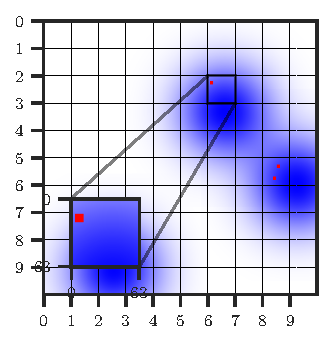
\includegraphics[scale=1.0]{figures/gaussian.pdf}
            \end{figure}
        \end{column}
    \end{columns}    
\end{frame}

\begin{frame}
    \frametitle{Environment II: Terrain}
    \begin{columns}
        \begin{column}{0.5\textwidth}
            \begin{itemize}
                \item Terrain seen from above (e.g. UAV).
                \item Targets between ocean and mountains.
                \item More realistic, higher variance.
            \end{itemize}
        \end{column}
        \begin{column}{0.5\textwidth}
            \begin{figure}
                \centering
                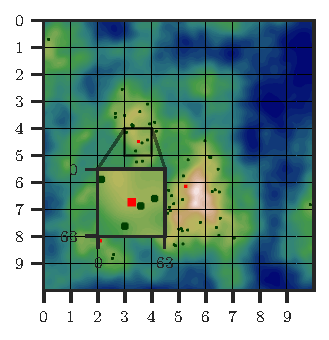
\includegraphics[scale=1.0]{figures/terrain.pdf}
            \end{figure}
        \end{column}
    \end{columns}   
\end{frame}

\begin{frame}
    \frametitle{Environment III: Camera}
    \begin{columns}
        \begin{column}{0.5\textwidth}
            \begin{itemize}
                \item Terrain seen from perspective projection camera.
                \item Moving actions control pan and tilt.
                \item Visually complex, difficult to interpret.
            \end{itemize}
        \end{column}
        \begin{column}{0.5\textwidth}
            \begin{figure}
                \centering
                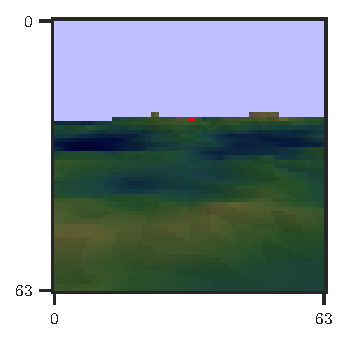
\includegraphics[scale=1.0]{figures/camera.pdf}
            \end{figure}
        \end{column}
    \end{columns}
\end{frame}

\subsection{Approach}

\begin{frame}
    \frametitle{Approach}

    \begin{itemize}
        \item Function approximation with deep neural networks:
        \begin{itemize}
            \item Policy \(\pi(a | s, \theta)\).
            \item Value \(v_\pi(s, \theta)\) (predicts future reward).
        \end{itemize}
        \item Training procedure:
        \begin{enumerate}
            \item Collect interactions with environment.
            \item Compute loss \(\mathcal{L(\theta)}\).
            \item Optimize \(\mathcal{L}\) wrt \(\theta\).
            \item Repeat\dots
        \end{enumerate}
        \item Loss function from proximal policy optimization~\cite{schulman_proximal_2017}.
        \begin{itemize}
            \item Relatively new RL algorithm.
            \item Stable performance, little hyperparameter tuning~\cite{henderson_deep_2018}
            \item May lead to non-global optima...
        \end{itemize}

    \end{itemize}
\end{frame}

\begin{frame}
    \frametitle{Architecture}

    \begin{figure}
        \centering
        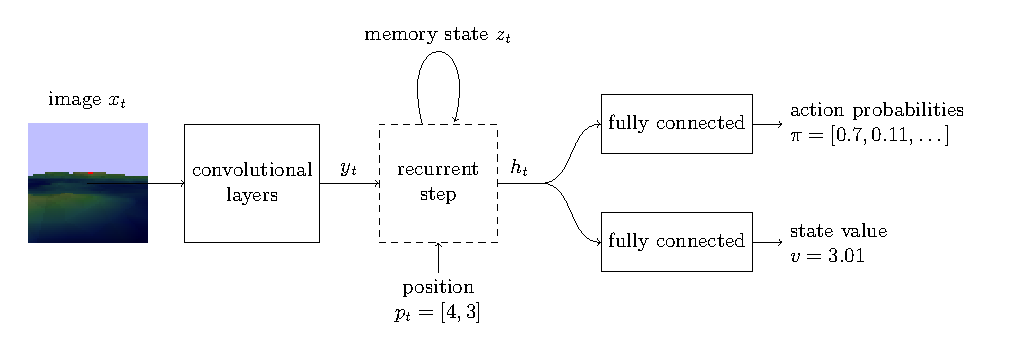
\includegraphics[scale=0.75]{figures/architecture-visual.pdf}
    \end{figure}

\end{frame}

\begin{frame}
    \frametitle{Memory}

    \begin{itemize}
        \item \textbf{Agent should remember visual features and associate them with their spatial location}.
        \item Two memory variants:
        \begin{enumerate}
            \item Temporal memory (long short-term memory~\cite{hochreiter_long_1997}):
            \begin{itemize}
                \item Previously applied to POMDPs \cite{hausknecht_deep_2017,mnih_asynchronous_2016,mirowski_learning_2017,gupta_cognitive_2019}.
                \item May struggle with remembering over many time steps.
                \item Important for exhaustive search and scene understanding.
            \end{itemize}
            \item Spatial memory (inspired by \cite{parisotto_neural_2017}):
            \begin{itemize}
                \item Map with one slot per camera position.
                \item Write image representation to current position memory.
                \item Read whole memory with convolutional layers.
            \end{itemize}
        \end{enumerate}
    \end{itemize}
\end{frame}

\begin{frame}
    \frametitle{Training}

    \begin{itemize}
        \item Train for 25M time steps.
        \item Results reported across 3 runs with different seeds.
        \item Separate training and test sets.
        \item Same hyperparameters in all runs.
    \end{itemize}
\end{frame}

\begin{frame}
    \frametitle{Implementation}

    \begin{itemize}
        \item OpenAI Gym environment interface.
        \item Custom PPO implementation.
        \item PyTorch for models and automatic differentiation.
        \item Intel Core i9-10900X CPU.
        \item NVIDIA GeForce RTX 2080 Ti GPU.
    \end{itemize}
\end{frame}